\chapter{Vývojová dokumentace}\label{ch:vyvojova-dokumentace}

Na začátku kapitoly popíšeme zvolené nástroje pro vývoj aplikace (sekce~\ref{sec:nastroje-pro-vyvoj}).
Také jsou zde popsány i řešení menších problémů, které si vyžadují vysvětlení jako je řešení autentizace, soukromí uživatelů apod.


\section{Nástroje pro vývoj}\label{sec:nastroje-pro-vyvoj}

V této sekci popíšeme nástroje a knihovny a vysvětlíme proč jsme se rozhodli je použít.
Projekt využívá continuous integration (CI), což je postup, kdy vývojáři projektu často (alespoň denně) integrují své změny do kódu projektu.
Tyto změny jsou provázeny kontrolní kompilací projektu a testováním, které pomáhají předejít chybám~\cite{ci-fowler}.
Projekt využívá CI konkrétně pro automatizování formátování kódu, statickou analýzu kódu, generování dokumentace a testování.
Jednotlivé části CI pipeline jsou detailně popsány níže.

\begin{description}
    \item[\href{https://github.com/features/actions}{GitHub Workflows}]
    Na základě dobré předchozí zkušenosti byl pro realizaci continuous integration zvolen nástroj Github Workflows.
    \item[\href{https://github.com/features/issues}{GitHub Issues}]
    Pro issue tracking byl zvolen nástroj GitHub Issues, který je přímo integrován do platformy GitHub.
    \item[\href{https://prettier.io/}{Prettier}]
    Standardizace formátování kódu zlepší čitelnost kódu a zrychlí vývoj~\cite{why-coding-style-matters}.
    Manuální formátování kódu je však zdlouhavé a proto použijeme nástroj, který tento proces automatizuje.
    Na základě osobní zkušenosti byl zvolen nástroj Prettier s jeho výchozím nastavením.
    \item[\href{https://eslint.org/}{ESLint}]
    Statická analýza kódu pomáhá předejít mnoha chybám a zvyšuje kvalitu kódu.
    Pro tyto účely jsem zvážil nástroj ESLint a \href{https://www.npmjs.com/package/jshint}{jshint}.
    Na základě pozitivní osobní zkušenosti s nástrojem ESLint a jeho vyššímu počtu týdenních stažení na npm registry byl zvolen nástroj ESLint~\cite{eslint, jshint}.
    \item[\href{https://codeql.github.com/}{CodeQL}]
    Statická analýza kódu může pomáhat předejít i bezpečnostním chybám.
    Proto jsme v projektu nasadili nástroj CodeQL, který je schopen detekovat bezpečnostní chyby pomocí sémantické analýzy kódu.
    Každá změna v kódu musí projít kontrolou tímto nástrojem než je sloučena do hlavní větve, pro zajištění maximální bezpečnosti.
    \item[\href{https://github.com/dependabot}{Dependabot}]
    Pravidelně probíhá kontrola všech závislostí nástrojem Dependabot, který upozorňuje na známé bezpečnostní chyby v závislostech.
    \item[\href{https://typedoc.org/}{TypeDoc}]
    Tento nástroj implementuje generování dokumentace z dokumentačních komentářů dle standardu \href{https://tsdoc.org/}{TSDoc}.
    Alternativou je \href{https://github.com/dotnet/docfx}{DocFX}, který je napsaný v jazyce C\#.
    Tento nástroj nemá npm balíček, což komplikuje integraci do našeho projektu.
    Pro tento projekt byl zvolen TypeDoc, jelikož implementuje stejný standard a jeho použití je v našem případě jednodušší.
    \item[\href{https://vitest.dev/}{Vitest}]
    Vývoj větších aplikací si vyžaduje testování kritických částí aplikace, abychom předešli špatné uživatelské zkušenosti a bezpečnostním chybám.
    Původně byla pro testování použita knihovna \href{https://jestjs.io/}{Jest}, ale konfigurace pro náš projekt byla neúspěšná.
    Složité chybové hlášky a nedostatečná dokumentace vedly na vykoušení jiné knihovnu.
    Byla zvolena knihovna Vitest, kterou bylo jednoduché nakonfigurovat zejména díky kvalitní dokumentaci.
    \item[\href{https://docusaurus.io/}{Docusaurus}]
    Součástí požadavků na tento projekt je také dokumentace.
    Dokumentace usnadňuje vývojářům orientaci v kódu a zachycuje důležitá rozhodnutí.
    Na začátku projektu byla využívána \href{https://docs.github.com/en/communities/documenting-your-project-with-wikis/about-wikis}{Github Wiki}, ale časem se ukázalo, že je pro tento projekt nevhodná.
    Github Wiki chybí podpora pro \textit{diagrams-as-code}\footnote{Diagrams-as-code je metoda pro tvorbu diagramů použitím textových definic zapsaných v doménově specifické jazyka~\cite{what-is-diagrams-as-code}} a také nelze zahrnout automaticky generovanou dokumentaci z kódu.
    Proto byly zváženy další alternativy jako \href{https://www.mkdocs.org/}{MkDocs}, \href{https://www.gitbook.com/}{GitBook} a \href{https://docusaurus.io/}{Docusaurus}.
    Docusaurus působí moderně, jednoduše a všechny jeho funkce jsou zdarma.
    Docusaurus má mnoho rozšíření jako například podporu pro diagramy jako kód.
    Docusaurus má oficiální plugin pro \href{https://mermaid.js.org/}{MermaidJS}, což je nástroj pro tvorbu diagramů.
    Ukázalo se, že MermaidJS není vhodný pro náš projekt, protože nemá dobrou podporu \href{https://c4model.com/}{diagramů C4 modelu}, které používáme pro dokumentaci architektury.
    Díky velkému ekosystému nástroje Docusaurus však existuje i komunitní plugin pro podporu \href{https://plantuml.com/}{PlantUML} diagramů, který má skvělou podporu diagramů C4 modelu.
    Integrace PlantUML diagramů s GitBook je naopak poměrně komplikovaná, proto GitBook nebyl použit.
    MkDocs a Docusaurus jsou srovnatelné, ale Docusaurus má některé funkce navíc jako např.\ použití React komponent pro tvorbu interaktivních částí.
    Přestože tyto funkce pravděpodobně nevyužijeme, nakonec byl zvolen nástroj Docusaurus.
\end{description}


\section{Soukromí uživatelů}\label{sec:soukromi-uzivatelu}

Aplikace pracuje s citlivými daty a proto je pro nás bezpečnost na prvním místě.
Tato sekce se věnuje krokům, které jsme podnikli pro zajištění maximální bezpečnosti a soukromí uživatelů.

Uživatelé v systému vystupují pod náhodně generovaným ID, aby i v případě úniku dat nebylo možné získat citlivé informace o uživatelích.

Po všech uživatelích vyžadujeme silná hesla, která jsou bezpečně uložena.
Pro řešení autentizace byly zváženy i bezheslové metody autentizace jako použití biometrických údajů, magic links či jednorázových tokenů~\cite{what-is-passworless}.
Tyto metody však nelze v naší aplikaci využít z následujících důvodů.
Chybí nám informace jako e\babelhyphen{nobreak}mail, telefonní číslo apod.
Nechceme po uživateli vyžadovat vlastnictví specializovaného hardware jako \href{https://cs.wikipedia.org/wiki/Bezpe%C4%8Dnostn%C3%AD_token}{bezpečnostní token} či skener otisku prstu.

Webové rozhraní používající knihovnu NextJS ve výchozím nastavení sbírá anonymní data o uživatelích~\cite{nextjs-telemetry}.
Na dotaz zadavatele byl sběr těchto dat vypnutý pro zvýšení důvěry uživatelů v platformu (viz produkční Dockerfile kontejneru \texttt{web-app}).

Dle vyjádření správců projektu Form.io software Form.io nesbírá žádná data o uživatelích~\cite{formio-telemetry-issue}.

\subsection{GDPR}\label{subsec:gdpr}

Při autentizaci uživatele používáme cookies pro správu session.
Ukládání dat do úložiště klienta spadá pod \href{https://eur-lex.europa.eu/eli/reg/2016/679/oj}{GDPR}, proto je nutno ověřit, jaké jsou naše povinnosti.
Dle \href{https://ec.europa.eu/justice/article-29/documentation/opinion-recommendation/files/2012/wp194_en.pdf}{doporučení Evropské Unie (sekce 3.2)} pro autentizační cookies je potřeba pro \emph{persistentní} cookies upozornit uživatele o jejich užití.
Knihovna NextAuth.js, kterou používáme má podporu pouze pro persistentní cookies (viz \href{https://github.com/nextauthjs/next-auth/issues/2534}{issue}), tedy musíme uživatele řádně upozornit.
Pro tento účel jsem zvolil knihovnu \href{https://www.npmjs.com/package/react-cookie-consent}{react-cookie-consent}.

GDPR také vyžaduje, aby uživatelé měli možnost smazat svá data.
Existuje však výjimka ohledně ukládání vědeckých dat.
% TODO: ověřit u NUDZ
Dle vyjádření NUDZ jsou veškerá data, která ukládáme slouží mimo jiné pro vědecké účely.


\section{Autentizace}\label{sec:auth}

Jak bylo vysvětleno v sekci~\ref{sec:soukromi-uzivatelu}, tak uživatelé se přihlašují pomocí náhodně generovaného ID a hesla.
Administrátoři se přihlašují pomocí e\babelhyphen{nobreak}mailu a hesla.
Pro autentizaci se používá knihovna NextAuth.js, která vykonává kód jak na klientovi, tak na serveru webové aplikace.
Tato knihovna má vlastní session management a vydává JWT tokeny.
Aby klient mohl pracovat se systémem spravující formuláře, je potřeba získat JWT token systému spravující formuláře.
Token systému spravující formuláře je vložen do tokenu vydávaného knihovnou NextAuth.js.
Tento systém zařizuje, že webová aplikace nemusí při každém požadavku od klienta komunikovat s systémem spravující formuláře, ale má vlastní session.
Kontrola práv uživatele při přístupu na ochráněnou stránku se kontrola provádí v middleware NextJS serveru.

\begin{figure}[H]
    \centering
    \includegraphics[width=0.9\textwidth]{diagrams/auth}
    \caption{Komunikace při autentizaci uživatele}\label{fig:auth}
\end{figure}


\section{Konfigurace a modifikace Form.io}\label{sec:konfigurace-a-modifikace-form.io}

\href{https://git-scm.com/book/en/v2/Git-Tools-Submodules}{Submodul} \texttt{/src/formio/} obsahuje fork projektu Form.io, kde bylo provedeno několik úprav.
Úpravy jsou poměrně malé a jejich cílem je přizpůsobit software našim potřebám.
Všechny změny jsou popsány v této sekci.
Dále jsou zde popsány některé části konfigurace Form.io.

\subsection{Modifikace}\label{subsec:modifikace}

\subsubsection{Inicializace projektu}\label{subsubsec:inicializace-projektu}

První úprava se týká inicializace instance při prvním startu.
Nepodařilo se najít způsob, jak nastavit inicializaci projektu tak, aby se automaticky vytvořili všechny potřebné zdroje (klient, pacient, zaměstnanec, apod.), role (admin, zaměstnanec, apod.).
Proto jsem upravil kód inicializace tak, aby se načetla z souboru \texttt{project.json} z kořenu repozitáře obsahující fork.
Původně se načítala z \texttt{project.json} v build složce, která však není uložena ve verzovacím systému.
Tato úprava byla nutná, jelikož nelze vytvářet nové role po inicializaci projektu a konfigurační soubor je nutné zahrnout do verzovacího systému.

\subsubsection{Webhook action}\label{subsubsec:webhook-action}

Webhook je koncept, který umožňuje poslat HTTP požadavek na zadanou URL jako reakci na určitou událost.
V našem případě se jedná o události jako je vytvoření nebo smazání formuláře.
V open-source verzi Form.io software je tato funkce podporována, ale neumí přeposílat hlavičky HTTP dotazu, který požadavek inicioval.
Tuto funkcionalitu potřebujeme, jelikož chceme přeposílat autentizační hlavičky při komunikaci mezi systémem spravující formuláře a systémem spravující úkoly uživatelů.
Detaily ohledně této komunikace jsou popsány v sekci~\ref{sec:propojeni-spravy-ukolu-a-spravy-formularu}.
Proto jsem upravil tuto funkci tak, aby bylo možné přeposílat autentizační hlavičky.

\subsubsection{Imutabilita ID uživatele}\label{subsubsec:imutabilita-id-uzivatele}

Form.io software lze rozdělit na dvě části.
První část je systém pro správu formulářu a sbírání odpovědí na tyto formuláře.
Druhá část je systém pro správu uživatelů.
Systém správy formulářů je použit i pro správu uživatelů systému.
V systému jsou vytvořeny registrační formuláře, které umožňují tvorbu uživatelských účtů.
Data o uživatelských účtech jsou pak uložena v uložišti odpovědí na tyto registrační formuláře.
V systému existují samosatné registrační formuláře pro různé role uživatelů.
My potřebujeme zajistit imutabilitu identifikátoru každého uživatele, který je uložen v položce \texttt{data.id}.
Motivaci k této změně naleznete v sekci~\ref{sec:auth}.
Databáze \href{https://www.mongodb.com/}{MongoDB}, která je použita pro ukládání dat o uživatelích neumí zajistit imutabilitu ukládaných dat.
Form.io však vždy přistupuje k databázi uživatelů skrze knihovnu \href{https://mongoosejs.com/}{Mongoose}.
Tato knihovna umí zajistit imutability zvolených položek.
Mongoose nastavíme tak, aby zajistil imutabilitu položky \texttt{data.id} (ID uživatele).
Pokud se uživatel pokusí změnit své ID v rámci úpravy svého profilu, tak se změna neprovede.
Nevýhodou tohoto řešení je, že vytváří omezení na položky \texttt{data.id} ve všech objektech reprezentující odevzdání, tedy i v těch, které nejsou uživatelské účty.

Alternativní řešení by bylo vytvořit autorizační proxy mezi klientem a Form.io serverem či mezi Form.io serverem a databází uživatelů.
Toto řešení by pravděpodobně vyžadovalo další kontejner a má netriviální implementaci.
Implementace by navíc měla nízkou odolnost vůči změnám.
Pokud bychom měli více koncových bodů API, které umožňují modifikovat entitu uživatele, bylo by potřeba myslet na zabezpečení všech koncových bodů.
V případě přidání nového bodu, by bylo vždy potřeba myslet na úpravy autorizační proxy.
Z těchto důvodů byla tato alternativa zavrhnuta a bylo použito řešení popsáno v předchozím odstavci.

\subsection{Konfigurace}\label{subsec:konfigurace}

Tato podsekce popisuje, jak byl software Form.io nakonfigurován pro náš projekt.

\subsubsection{Konfigurace zdrojů (resources)}\label{subsubsec:konfigurace-resources}

Form.io pracuje s konceptem zdrojů, které lze zjednodušeně chápat jako kolekce objektů v databázi.
Detailní popis tohoto konceptu lze nalézt v \href{https://help.form.io/userguide/resources}{dokumentaci Form.io}.
Pro nás je nyní důležité, že každý objekt patří do právě jednoho zdroje.
Toto omezení platí, protože používáme bezplatnou verzi Form.io.
Uživatelé jsou reprezentováni jako objekty patřící do nějakého zdroje.
Každý zdroj je svázán se sadou rolí.
Role uživatele jsou tedy určeny zdrojem, kterému uživatel patří.
Proto je potřeba vytvořit zdroj pro každou kombinaci rolí, které může uživatel mít.
Vzhledem k tomu, že jsou tyto zdroje oddělené, nelze při tvorbě uživatelského účtu jednoduše validovat, že má každý uživatel unikátní ID pro přihlášení.
Abychom předešli zmatení uživatelů, v uživatelském rozhraní vždy k ID přidáme i roli, která je uživateli přiřazena.

Alternativně bychom mohli každé existující kombinaci rolí přidat prefix do ID uživatele.
Toto řešení však značně zhoršuje uživatelskou přívětivost a proto nebylo použito.


\section{Propojení správy úkolů a správy formulářů}\label{sec:propojeni-spravy-ukolu-a-spravy-formularu}

Náš systém obsahuje komponentu spravující úkoly a komponentu spravující formuláře.
Každý úkol je spojen s formulářem, který má uživatel vyplnit.
Potřebujeme v našem distribuovaném systému zajistit, aby uživatel mohl vyplnit dotazník pouze tehdy, když má úkol na jeho vyplnění.
Popíšeme dvě možnosti řešení tohoto problému a následně zvolíme jednu z nich.

První možností řešení je, že uživatel vyplní dotazník a \emph{odešle se požadavek na komponentu spravující formuláře}, kde je připraven webhook, který proběhne \emph{před} uložením výsledku, kde proběhne kontrola existence úkolu na vyplnění tohoto dotazníku.
Pokud úkol existuje, tak se vyplnění dotazníku uloží společně s identifikátorem úkolu a také se splní úkol a uloží se k němu identifikátor vyplnění dotazníku.
V případě, že úkol neexistuje, tak se vyplnění dotazníku neuloží a uživatel je informován o chybě.
Dotazník obsahuje skryté pole, které obsahuje identifikátor úkolu v rámci, kterého byl dotazník vyplněn.
Tím je zajištěno, že vyplnění dotazníku drží informaci o identifikátoru úkolu v rámci kterého byl vyplněn.

Zvažme nyní druhou možnost řešení.
Uživatel vyplní dotazník a \emph{odešle se požadavek na komponentu spravující úkoly}, která za něj dotazník odevzdá pokud má uživatel úkol na jeho vyplnění.
Situace se při tomto řešení komplikuje, jelikož bychom museli zajistit, že všechny požadavky na vyplnění dotazníku musí jít skrze komponentu spravující úkoly.
Museli bychom tedy zakázat, aby uživatel odevzdal dotazník přímo do systému spravující formuláře.
Kdybychom to neudělali, tak nejsme schopni zajistit integritu sesbíraných dat.
Toto omezení bychom mohli zajistit úpravou konfigurace reverse proxy, kterou prochází všechny požadavky z vnějšího světa, nebo úpravou systému spravující formuláře.
První zmíněný způsob by však nezajistil ochranu před požadavky z vnitřní sítě.
Pro ochranu před požadavky z vnitřní sítě je lepší druhý způsob.
Systém spravující formuláře je řešením třetí strany a vyžadovalo by to zásah do jejich kódu.

Zvolíme první alternativu, jelikož je jednodušší na implementaci a má dobré vlastnosti.
Nyní si rozmysleme detaily implementace.
Chceme zajistit, aby se nám nepodařilo vytvořit více vyplnění dotazníku pro stejný úkol.
Proto formulář, který bude zadáván jako úkol pro plnitele, nastavíme tak, aby zajistil unikátnost hodnoty skryté položky obsahující identifikátor úkolu.
Nyní popíšeme celý proces vyplnění dotazníku formou diagramu (Obr.~\ref{fig:activity-diagram-task-and-form-integration}) používající \href{https://www.bpmn.org/}{Business Process Model and Notation}.

\begin{figure}[H]
    \centering
    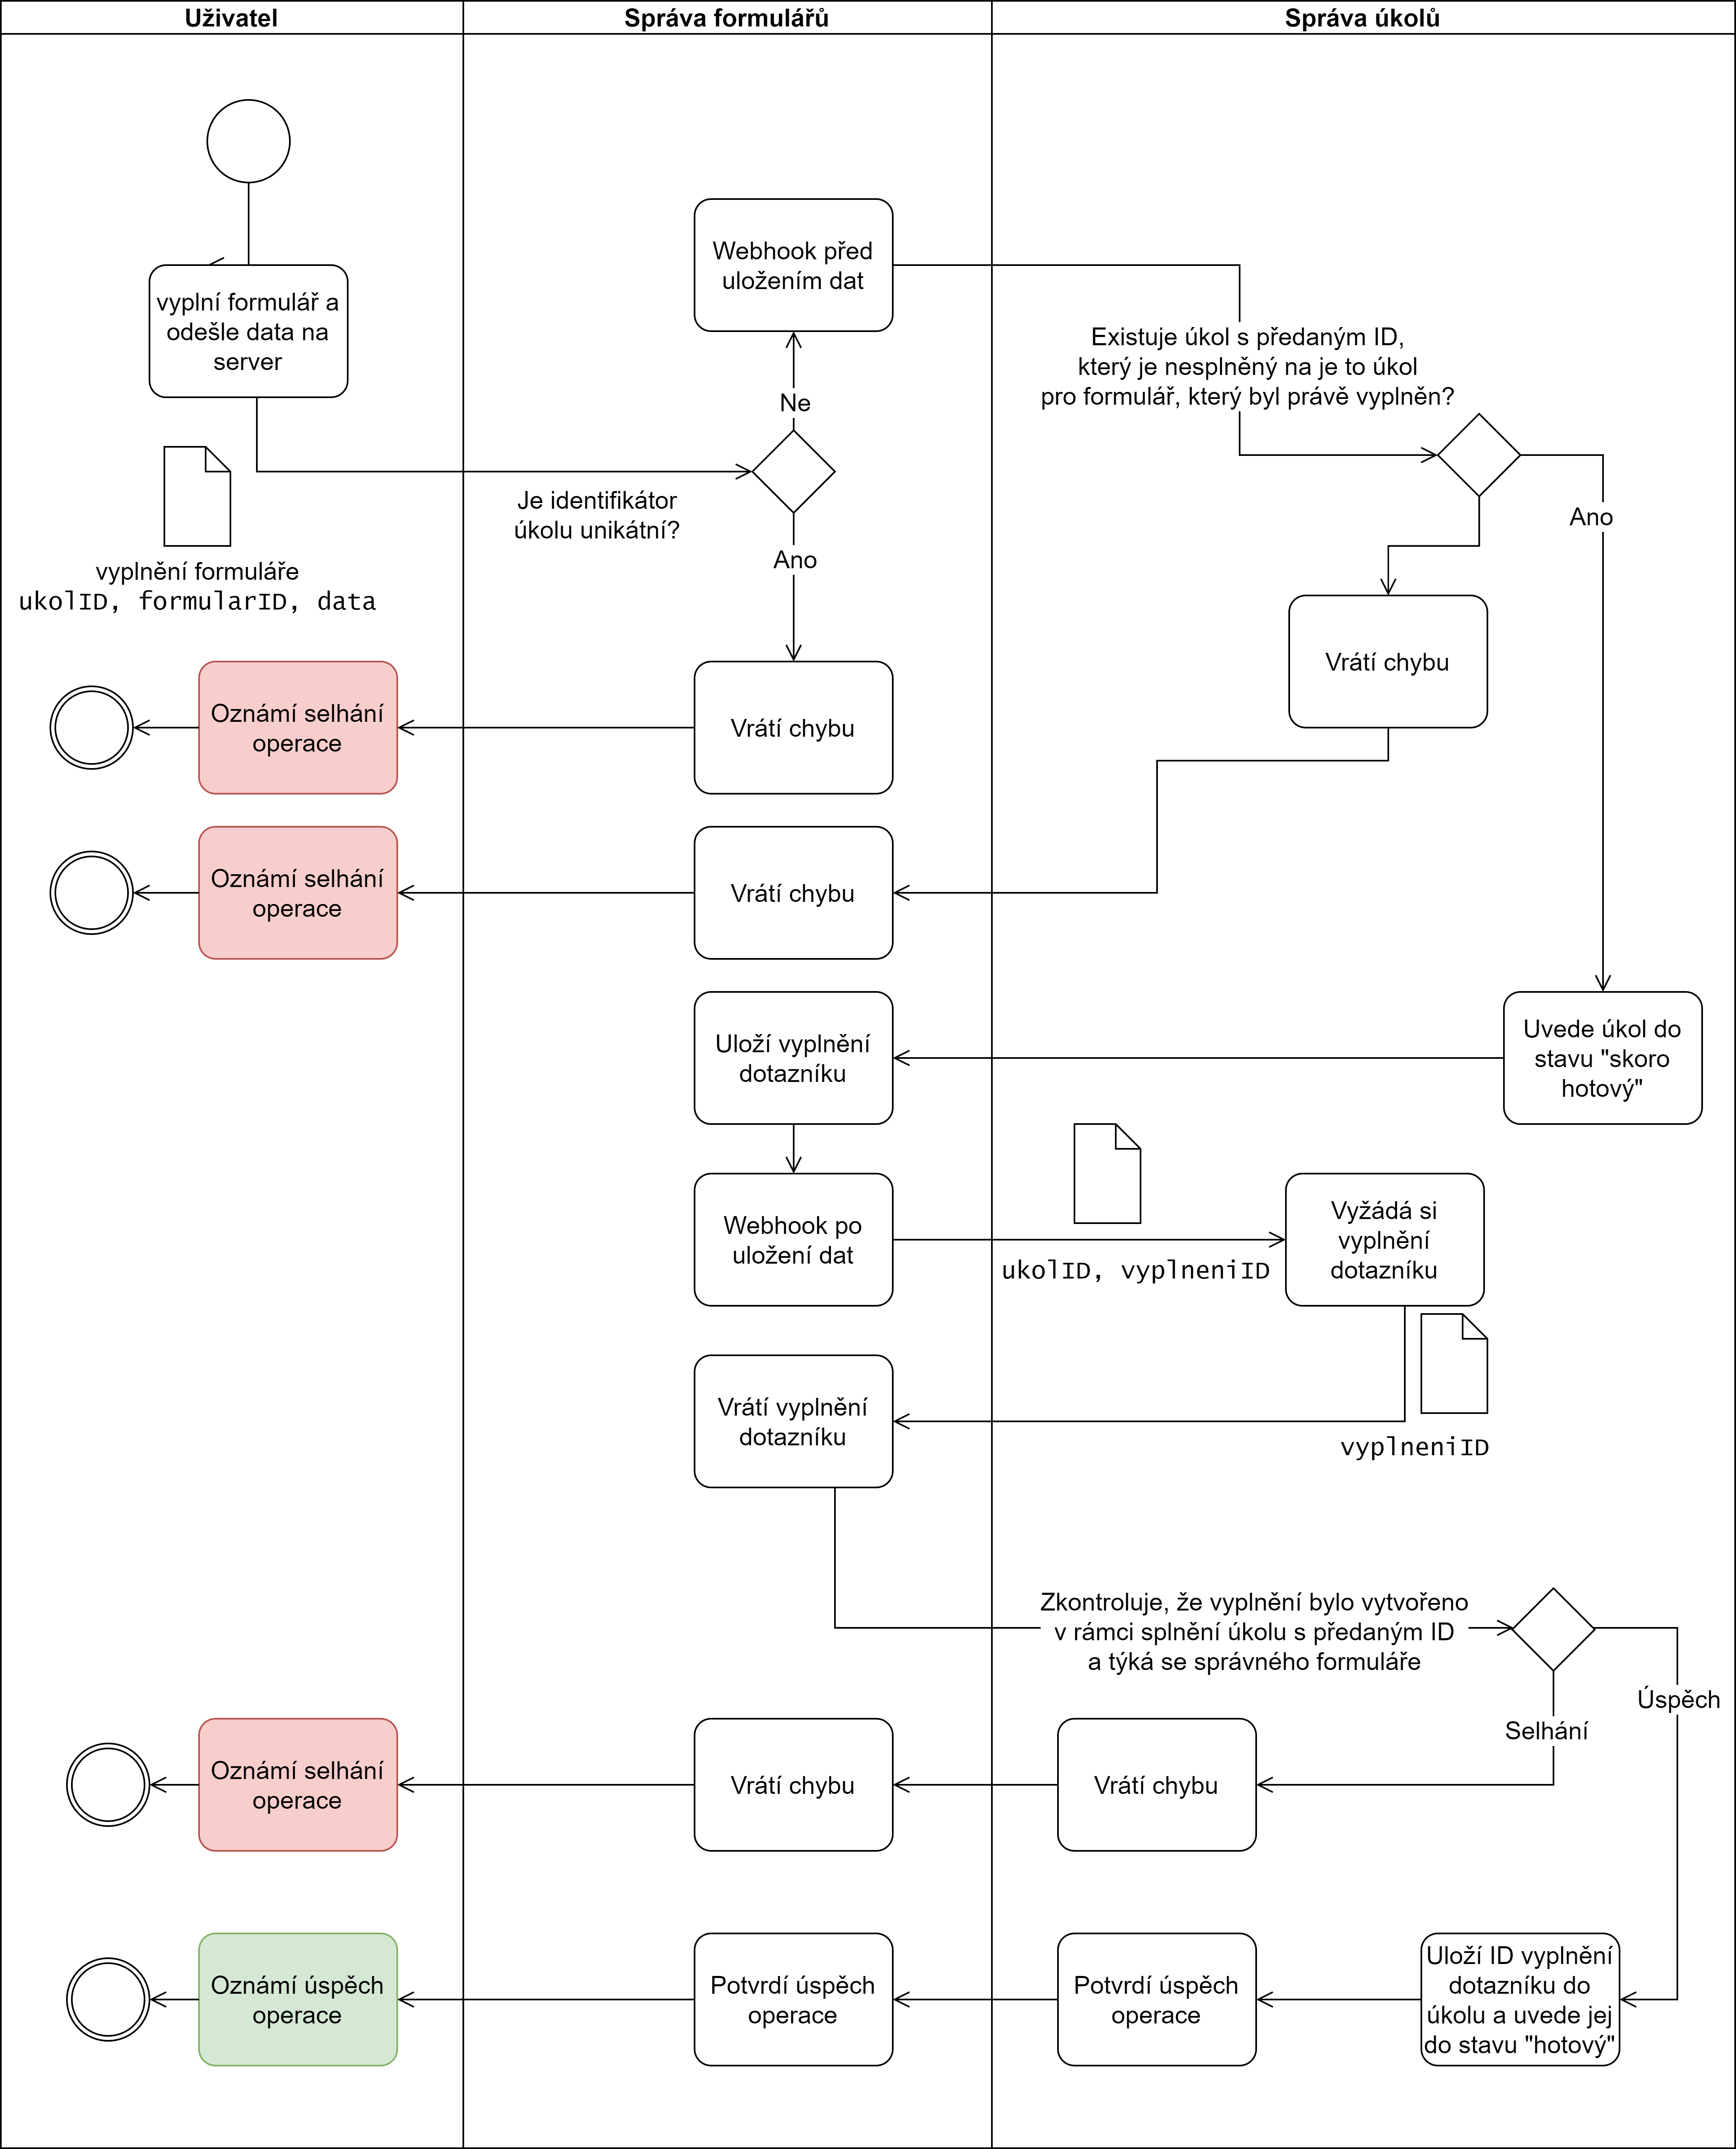
\includegraphics[width=\textwidth]{diagrams/activity.drawio}
    \caption{Diagram integrace systémů spravující úkoly a systému spravující formuláře}\label{fig:activity-diagram-task-and-form-integration}
\end{figure}

Požadavek na uložení vyplnění dotazníku spustí webhook.
V rámci reakce na tento webhook uvedeme úkol do stavu \texttt{skoro hotový}.
Tento stav slouží k tomu, aby nebylo možné vytvořit další vyplnění dotazníku v rámci stejného úkolu.
Tento mechanismus se nazývá \emph{semantic lock counter-measure}~\cite{semantic-lock-countermeasure-def}.
Stavy úkolu a přechody mezi nimi jsou popsány stavovým diagramem v jazyce UML na obr.~\ref{fig:task-state}.

Nyní popíšeme, jak je tento mechanismus využíván v našem systému.
Pokud požadavek na uložení vyplnění dotazníku spustí webhook, který proběhne před uložením do systému spravující formuláře, a následně selže operace uložení vyplnění dotazníku v systému spravující formuláře, tak úkol navždy zůstane ve stavu \texttt{skoro hotový}.
Pokud bychom se z tohoto stavu chtěli dostat, potřebovali bychom implementaci \href{https://microservices.io/patterns/data/saga.html}{ság}, která by zajistila provedení kompenzačních transakcí.
Popsaná situace je však natolik výjimečná, že se v tuto chvíli problematice věnovat nebudeme.
Vystačíme si s tím, že systém spravující formuláře nikdy nebude obsahovat vyplnění dotazníku, které vzniklo bez zadání úkolu.

\begin{figure}[H]
    \centering
    \includegraphics[width=0.9\textwidth]{diagrams/taskState}
    \caption{Stavový diagram úkolů}\label{fig:task-state}
\end{figure}

Po uložení vyplnění dotazníku se zavolá druhý webhook, který zařídí uložení informace o identifikátoru vyplnění do úkolu.
Vzhledem k tomu, že se jedná o veřejně dostupný endpoint, tak je nutné ověřit poskytnutá data.
Musíme si tedy z úkolového systému vyžádat vyplnění dotazníku a zkontrolovat všechny náležitosti.
Pokud by se někdo pokusil spárovat úkol s formulářem, který je ve stavu \texttt{skoro hotový} na jiné vyplnění dotazníku než to, které způsobilo přechod úkolu do stavu \texttt{skoro hotový}, tak operace jistě selže.
Kdyby se někdo pokusil spárovat úkol s vyplněním dotazníku, který neodpovídá dotazníku zadaný úkolem, tak operace jistě selže.
V případě, že by se někdo pokusil spárovat jiné vyplnění stejného dotazníku, tak se mu to také nepovede.
Ono jiné vyplnění dotazníku by muselo mít jiný identifikátor úkolu v skrytém poli, protože systém spravující formuláře zajišťuje unikátnost těchto hodnot.
Jelikož víme, že již existuje vyplnění dotazníku, které má identifikátor úkolu v skrytém poli stejné jako identifikátor úkolu, který se právě snažíme napárovat, tak víme, že jakékoliv jiné vyplnění stejného dotazníku bude mít jiný identifikátor úkolu v skrytém poli.

\paragraph{Autentizace webhooků}

HTTP požadavky, které dělá systém spravující formuláře při tvorbě odevzdání formuláře na systém spravující úkoly, musí obsahovat autentizační hlavičky.
První možností je poskytnout systému spravující formuláře speciální přístupový token.
Toto však nelze provést pouze pro některé webhooky bez většího zásahu do zdrojového kódu systému spravující formuláře, ale pouze pro všechny webhooky najednou.
Navíc to situaci zbytečně komplikuje.

Druhá možnost je využití JWT tokenu z požadavku na vytvoření odevzdání formuláře, který je přijat systémem spravující formuláře.
Toto je dobrá možnost, ale open-source verze systému spravující formuláře tuto funkci nemá.
Nicméně není těžké ji do něj přidat.

Třetí možností je vyhnout se autentizaci webhooku pomocí přihlášení.
Místo toho bychom mohli vytvořit endpoint komponenty spravující úkoly, který je přístupný pouze z komponenty spravující formuláře.
Toto však znamená netriviální úpravy síťové infrastruktury.
Tyto úpravy jsou poměrně špatně udržovatelné.

Použijeme druhou možnost, jelikož má jednoduchou implementaci.
Provedené úpravy systému spravující formuláře jsou popsány v sekci~\ref{sec:konfigurace-a-modifikace-form.io}.

